\cleardoublepage
\chapter{Solaio}\label{chap:solaio}
Il solaio da progettare è quello rappresentato in figura~\ref{fig:solaioPianoSecondo} di pagina~\pageref{fig:solaioPianoSecondo} ed è composto da due campate di luce pari a $4.00\,m$ e $5.00\,m$. Dall'analisi dei carichi effettuata al punto~\ref{sec:azioniSolaio} di pagina~\pageref{sec:azioniSolaio} sono stati ricavati i valori delle caratteristiche di sollecitazione sulle sezioni di maggior interesse; le tabelle~\ref{tab:bendingMoment_solaio} e \ref{tab:shear_solaio} sintetizzano quanto appena detto in riferimento a una striscia di solaio di larghezza pari a $1\,m$.

\section{Progetto e verifica agli SLU per tensioni normali}\label{sec:solaioBendingMoment_slu}

La scelta dell'altezza del solaio strutturale può essere effettuata usando una semplice formula approssimativa
\[
H = \dfrac{1}{25}\,\max\{l_i\} = \dfrac{1}{25}\,\max\{4.00; 5.00\}\,m = \dfrac{5.00\,m}{25} = 0.20\,m = 200\,mm
\]

Si sceglie, a favore di sicurezza, un solaio $20+4\,cm$ costituito da una pignatta di altezza $20\,cm$ e da una soletta gettata in opera di $4\,cm$. L'interassi $i$ dei travetti è costante e pari a $50\,cm$. Ricapitolando, le caratteristiche geometriche del solaio sono
\begin{align*}
    H &= 240\,mm\\
	s &= 40\,mm\\
	B &= i = 500\,mm\\ 
	d' &= d'' = 40\,mm\\
	d &= H - d' = 200\,mm\\
	b &= 120\,mm
\end{align*}
dove $b$ è la larghezza del travetto. Le caratteristiche dei materiali sono quelle utilizzate per la trave e per il pilastro. Di seguito si riportano il progetto e la verifica agli SLU per tensioni normali sulle sezioni di specifica rilevanza.

In continuità con la notazione usata nel capitolo~\ref{sec:azioniSolaio} la campata $1$ verrà denominata $CS1$, la campata $2$ come $CS2$ e l'appoggio che divide le due campate come $NS2$.

\subsection{Sezione CS1}\label{sec:sezioneCS1}
\subsubsection{Progetto}

In campata il momento massimo positivo \emph{per un metro di solaio} vale
\[
M_{Ed}^{CS1} = 30.06\,kN\,m
\]
e si raggiunge all'ascissa $s = 2.07\,m$. Volendo progettare un singolo travetto di interasse $i=50\,cm$, si deve considerare solo metà del momento flettente sopra riportato; il momento sollecitante di progetto che grava sul travetto vale
\[
M_{Ed}^{CS1} = 15.03\,kN\,m
\]

Come ipotesi iniziali si assume che l'\emph{asse neutro tagli l'ala} e che $\epsilon_c \leq \epsilon_{c2}$. Usando il legame costitutivo parabola rettangolo, nell'ipotesi di essere in campo 2, per il calcestruzzo si ha
\[
\psi = \dfrac{\xi}{1-\xi}\,\dfrac{\epsilon_{su}}{3\,\epsilon_{c2}^2}\,\left(3\,\epsilon_{c2} - \dfrac{\xi}{1-\xi}\,\epsilon_{su}\right)
\]
e
\[
\lambda = \dfrac{4\,\epsilon_{c2} - \dfrac{\xi}{1-\xi}\,\epsilon_{su}}{4\,\left(3\,\epsilon_{c2}-\dfrac{\xi}{1-\xi}\,\epsilon_{su}\right)}
\]
dove $\xi = \frac{x}{d}$ è la posizione dell'asse neutro adimensionalizzata. Dall'equilibrio alla traslazione si ricava la posizione dell'asse neutro specificata in funzione dell'area di armatura, mentre dall'equilibrio alla rotazione attorno a punto di applicazione delle compressioni nel calcestruzzo si calcola il valore di $A_s$ e quindi di $\xi$. Il sistema risolvente è perciò

\[
\begin{cases}
	B\,\psi\,\xi\,d\,f_{cd} - A_s\,f_{yd}= 0\\
	A_s\,f_{yd}*(d - \lambda\,xi\,d) = M_{Ed}^{CS1}
\end{cases}
\]
da cui si ricava
\begin{align*}
    \xi &= 0.11448~\Longrightarrow~x = \xi\,d = 22.28\,mm < s = 40\,mm\\
	A_s &= 200.79\,mm^2~\Longrightarrow~A_s = 2\,\Phi\,12\,mm = 72\,\pi\,mm^2 = 226.195\,mm^2
\end{align*}

L'ipotesi di asse neutro che taglia l'ala è corretta; l'ipotesi sul calcestruzzo si verifica come
\[
\dfrac{\epsilon_{su} + \epsilon_c}{d} = \dfrac{\epsilon_c}{x}
\]

Risolvendo si ricava
\[
\epsilon_c = 1.2928\,\permil < \epsilon_{c2}
\]
che è coerente con quanto assunto sopra. Ulteriore verifica è sulla base minima del travetto
\[
b_{min} = 2\,c + n\,\Phi + (n-1)\,s_{min} = 2\cdot 10\,mm + 2\cdot 12\,mm + 1\cdot 25\,mm = 69\,mm < b = 120\,mm
\]

\subsubsection{Verifica}
Con le ipotesi fatte in precedenza e utilizzando il quantitativo di armatura scelto sopra, si deve verificare l'effettiva posizione dell'asse neutro; dall'equilibrio alla traslazione
\[
B\,\psi\,\xi\,d\,f_{cd} - A_s\,f_{yd} = 0
\]
da cui si ricava
\[
    \xi = 0.1192~\Longrightarrow~x = \xi\,d = 23.84\,mm < s = 40\,mm
\]

L'asse neutro taglia l'ala come previsto. La deformazione del calcestruzzo con il valore di $\xi$ appena trovato vale
\[
    \epsilon_c = 1.353\,\permil
\]
che è compatibile con quanto assunto. Si calcolano i valori di $\psi$ e $\lambda$ che valgono
\[
    \psi = 0.5240
\]
\[
    \lambda = 0.3576
\]

Il momento resistente della sezione vale
\begin{equation}
	M_{Rd}^{CS1} = B\,\psi\,\xi\,d\,f_{cd}\,\left(d - \lambda\,\xi\,d\right) = 16.95\,kN\,m > M_{Ed}^{CS1} = 15.03\,kN\,m
\end{equation}

\subsection{Sezione NS2}
\subsubsection{Progetto}
Trovandosi su un appoggio la sezione è ribaltata; questo implica che le ali si trovano in trazione e perciò non danno contributo lato calcestruzzo. Non si pone, quindi, il problema di dove si posizioni l'asse neutro -  che taglierà necessariamente l'anima.

Il momento sollecitante sul travetto vale
\[
M_{Ed}^{NS2} = 18.47\,kN\,m
\]
che coincide con il massimo momento flettente in valore assoluto. Si suppone che il calcestruzzo sia a collasso, per cui
\[
    \psi = 0.80952
\]
e 
\[
    \lambda = 0.416
\]

Dall'equilibrio alla rotazione
\[
b\,\psi\,\xi\,d\,f_{cd}\,\left(d-\lambda\,\xi\,d\right) = M_{Ed}^{NS2}
\]
si ricava $\xi$
\[
    \xi = 0.4031~\Longrightarrow~x = 80.61\,mm
\]
Le armature inferiori hanno deformazione pari a 
\[
\epsilon_s = 5.1834\,\permil > \epsilon_{se}
\]
il che garantisce la plasticizzazione delle stesse. L'area di armatura necessaria si calcola dall'equilibrio alla traslazione e risulta
\[
    A_s = 283.58\,mm^2~\Longrightarrow~A_s = 3\,\Phi\,12\,mm = 108\,\pi\,mm^2 = 339.292\,mm^2
\]

La base minima
\[
b_{min} = 2\cdot 10\,mm + 3\cdot 12\,mm + 2\cdot 25\,mm = 106\,mm < b = 120\,mm
\]

\subsubsection{Verifica}
Nell'ipotesi che il calcestruzzo compresso si trovi a collasso con $\psi$ e $\lambda$ costanti e pari a quelli adottati durante il progetto, sviluppando l'equilibrio alla traslazione
\[
b\,\psi\,\xi\,d\,f_{cd} - A_s\,f_{yd} = 0
\]
e isolando $\xi$
\[
    \xi = 0.4823~\Longrightarrow~x = 96.45\,mm
\]
da cui si deduce che il calcestruzzo si trova in campo 3 ($\xi\in [0.2593, 0.6526]$). Inoltre, l'asse neutro si trova circa a metà sezione. La deformazione dell'armatura tesa è
\[
\epsilon_s = 3.757\,\permil > \epsilon_{se}
\]
cioè è snervata. Le ipotesi progettuali sono corrette e il momento resistente vale
\begin{equation}
	M_{Rd}^{NS2} = b\,\psi\,\xi\,d\,f_{cd}\,\left(d - \lambda\,\xi\,d\right) = 21.23\,kN\,m > M_{Ed}^{NS2} = 18.47\,kN\,m
\end{equation}

\subsection{Sezione CS2}
\subsubsection{Progetto}
In campata 2 la sezione è nuovamente a $T$ e si ripropone il problema di dove si posiziona l'asse neutro. Si assume l'ipotesi tale per cui l'asse neutro taglia l'ala. Il momento sollecitante sul travetto è
\[
M_{Ed}^{CS2} = 8.63\,kN\,m
\]
e si supponga, come per la campata $CS1$, che il calcestruzzo abbia deformazione 
\[
\epsilon_c \leq \epsilon_{c2}
\]

Con questo range di valore di deformazione si hanno
\begin{align*}
	\psi &= \dfrac{\xi}{1-\xi}\,\dfrac{\epsilon_{su}}{3\,\epsilon_{c2}^2}\,\left(3\,\epsilon_{c2} - \dfrac{\xi}{1-\xi}\,\epsilon_{su}\right)\\
	\lambda &= \dfrac{4\,\epsilon_{c2} - \dfrac{\xi}{1-\xi}\,\epsilon_{su}}{4\,\left(3\,\epsilon_{c2}-\dfrac{\xi}{1-\xi}\,\epsilon_{su}\right)}
\end{align*}
e sostituendole nell'equilibrio alla rotazione e isolando $\xi$ si ottiene
\[
\xi = 0.08225~\Longrightarrow~x = 16.45\,mm
\]

L'asse neutro si trova molto in alto e perciò taglia necessariamente l'ala del travetto. Trovandosi in campo 2 la crisi dei materiali è lato acciaio (teso). La deformazione del calcestruzzo vale
\[
\epsilon_c = 0.8962\,\permil < \epsilon_{c2}
\]
coerentemente con quanto assunto sopra. Dall'equilibrio alla traslazione si calcola l'area di armatura necessaria
\[
    A_s = 113.52\,mm^2~\Longrightarrow~A_s = 2\,\Phi\,12\,mm = 72\,\pi\,mm^2 = 226.195\,mm^2
\]

Il calcolo della base minima è analogo a quello eseguito per la campata $CS1$.

\subsubsection{Verifica}
Con i valori di $\psi$ e $\xi$ riportati nel progetto della sezione $CS2$ si calcola la posizione dell'asse neutro effettiva (con riferimento all'armatura realmente inserita), risolvendo l'equilibrio alla traslazione 
\[
    \xi = 0.1192~\Longrightarrow~x = 23.84\,mm < s = 40\,mm
\]

L'asse neutro taglia l'ala. La deformazione del calcestruzzo è
\[
\epsilon_c = 1.3533\,\permil < \epsilon_{c2}
\]
che è compatibile con quanto ipotizzato. La sezione si trova in campo 2; i parametri del calcestruzzo hanno i seguenti valori
\begin{align*}
    \psi&= 0.5240\\
	\lambda &= 0.3576
\end{align*}

Il momento resistente della sezione è
\begin{equation}
	M_{Rd}^{CS2} = B\,\psi\,\xi\,d\,f_{cd}\,\left(d - \lambda\,\xi\,d\right) = 16.95\,kN\,m > M_{Ed}^{CS2} = 8.63\,kN\,m
\end{equation}

Come previsto, la sezione ha caratteristiche geometriche e meccaniche pari alla sezione $CS1$.
\begin{figure}
    \centering
	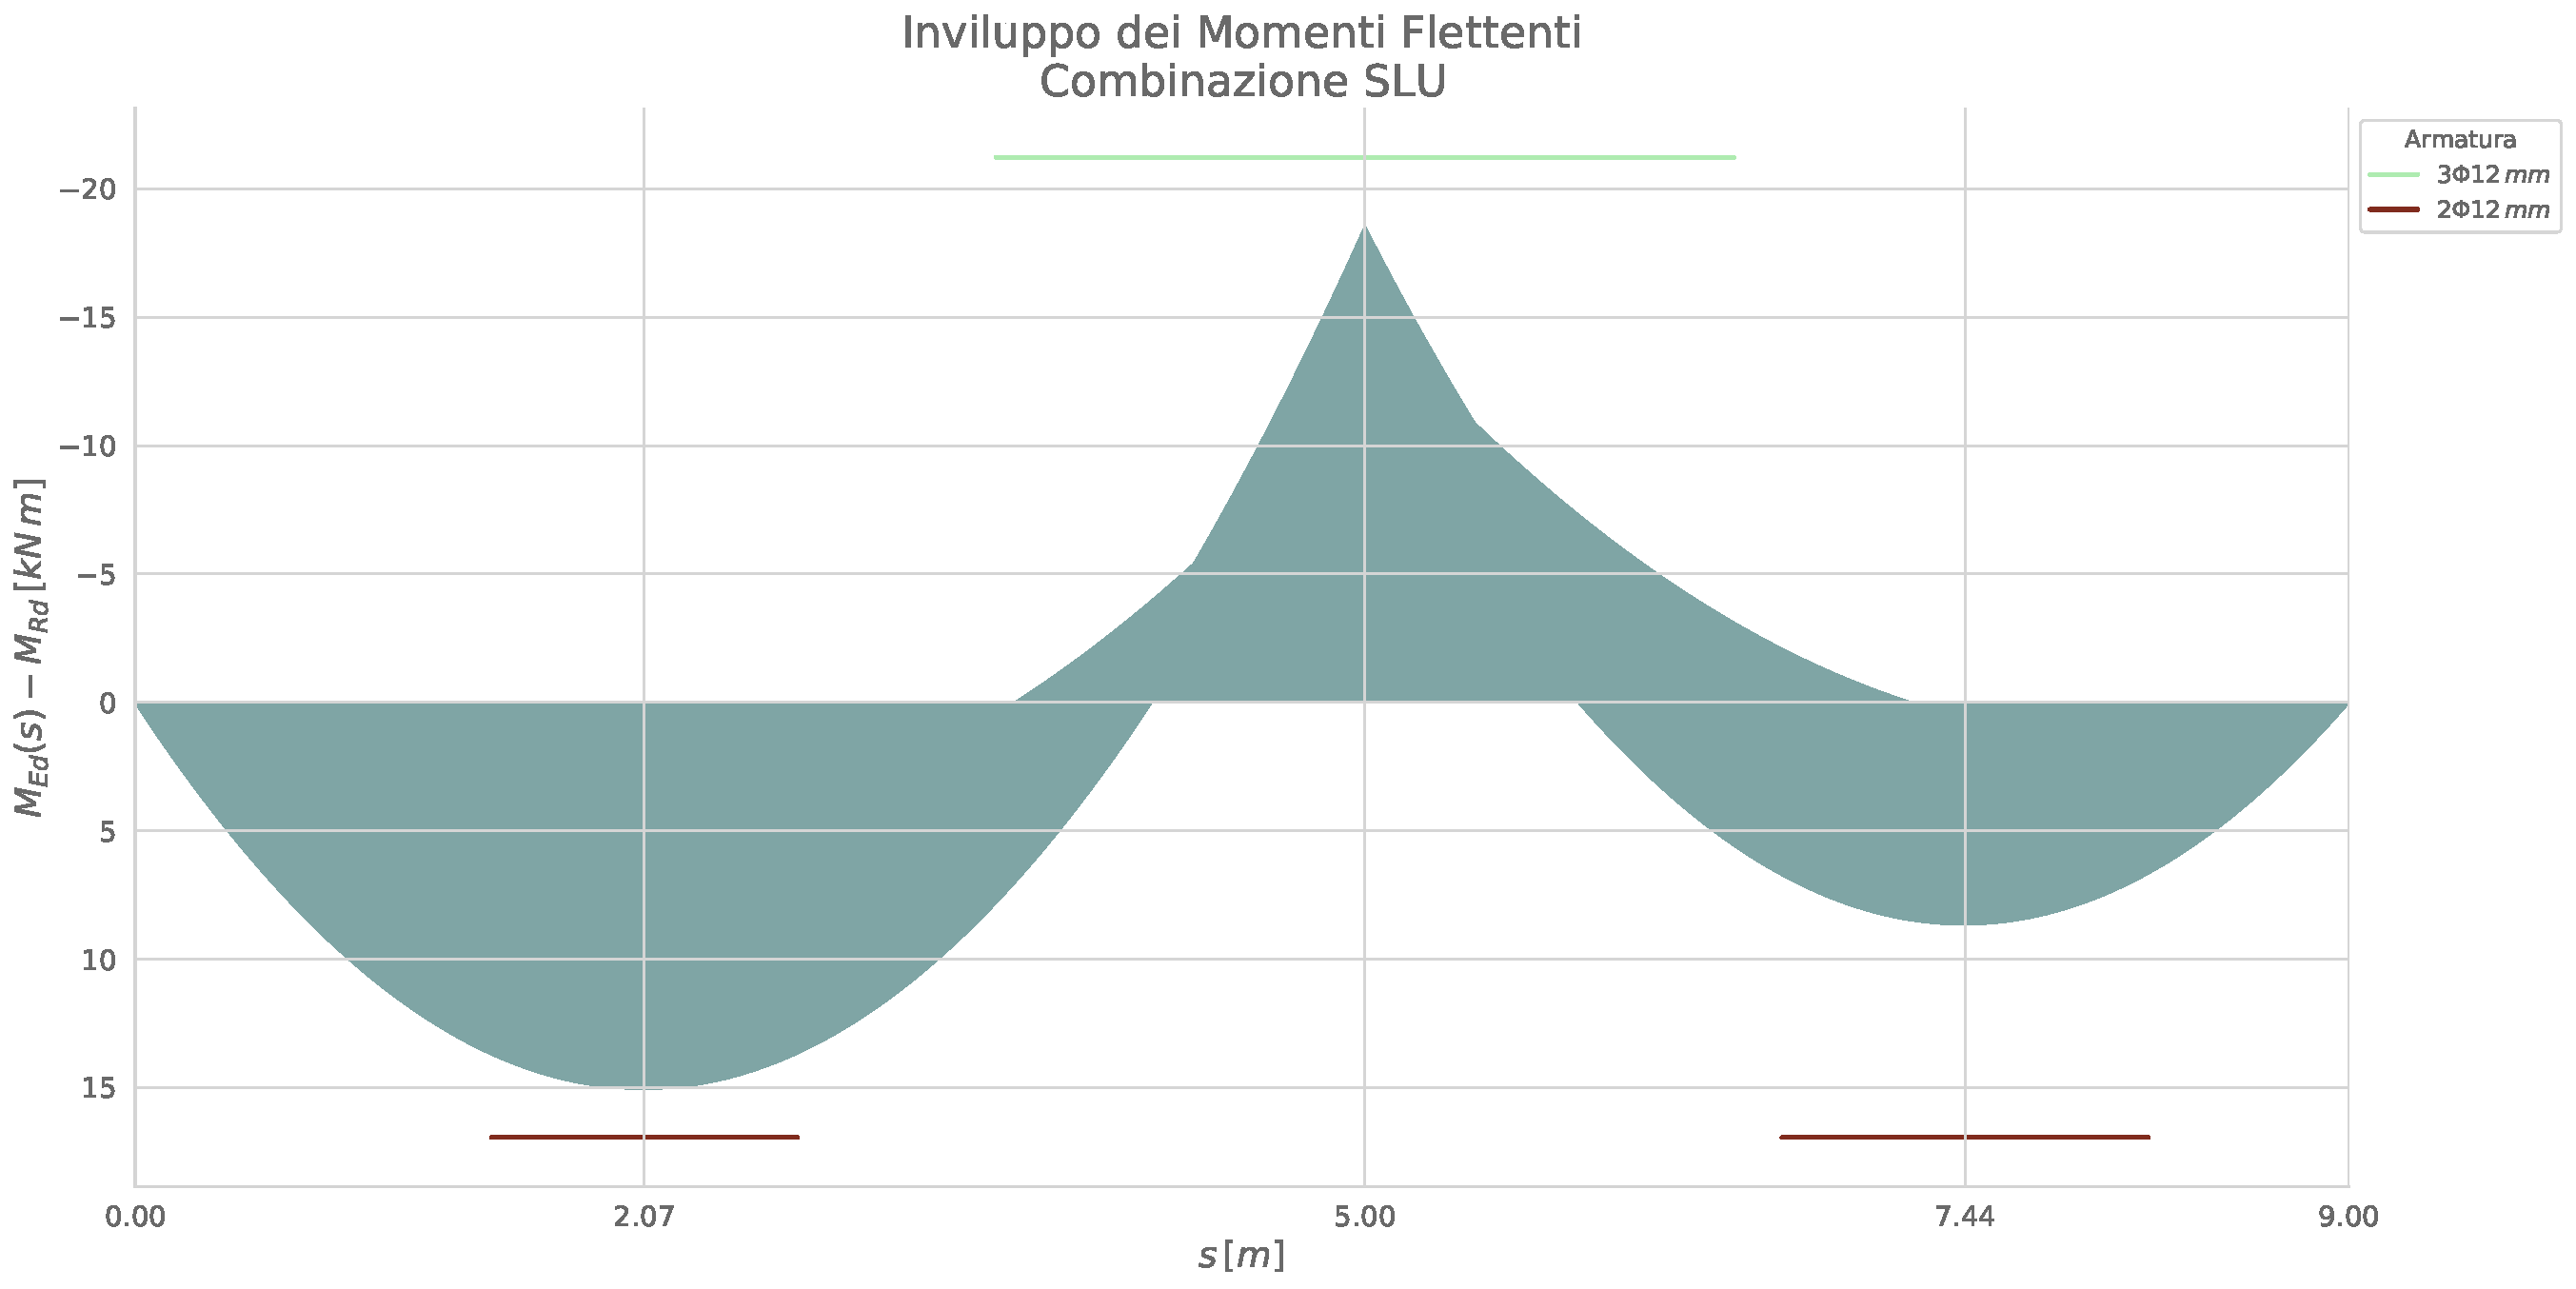
\includegraphics[width=\textwidth]{MEd-MRd_solaio}
	\caption{Sovrapposizione momento sollecitante e momento resistente -- solaio}
	\label{fig:MEd-MRd_solaio}
\end{figure}

\cleardoublepage
\section{Verifica sulle armature}
La verifica sul quantitativo di armature va eseguita parallelamente a quanto fatto per la trave. L'area minima di armatura da inserire nel travetto è
\[
A_{s,min} = \max\left\{0.26\,\dfrac{fctm}{fyk}\,b_t\,d; 0.0013\,b_t\,d\right\} = 35.57\,mm^2
\]
che è soddisfatta, avendo scelto $2\,\Phi\,12\,mm = 226.195\,mm^2$. L'area di armatura massima, invece
\[
A_{s,max} = 0.04\,A_c = 1760\,mm^2  
\]
anch'essa soddisfatta.

\section{Traslazione del diagramma dei momenti flettenti }\label{sec:traslazioneSolaio}
Come per la trave, anche per il solaio è necessario traslare il diagramma dei momenti flettenti in modo da assorbire l'azione del taglio. La traslazione avviene secondo quanto applicato per la trave, con la sola differenza che non può essere applicata armatura a taglio; si ha perciò
\[
    a_1 = 0.9\,d = 0.9\cdot 200\,mm = 180\,mm
\]

Riportandolo sul diagramma si ottiene quanto rappresentato in figura~\ref{fig:MEd-MRd_traslato_solaio}.

\begin{figure}
    \centering
	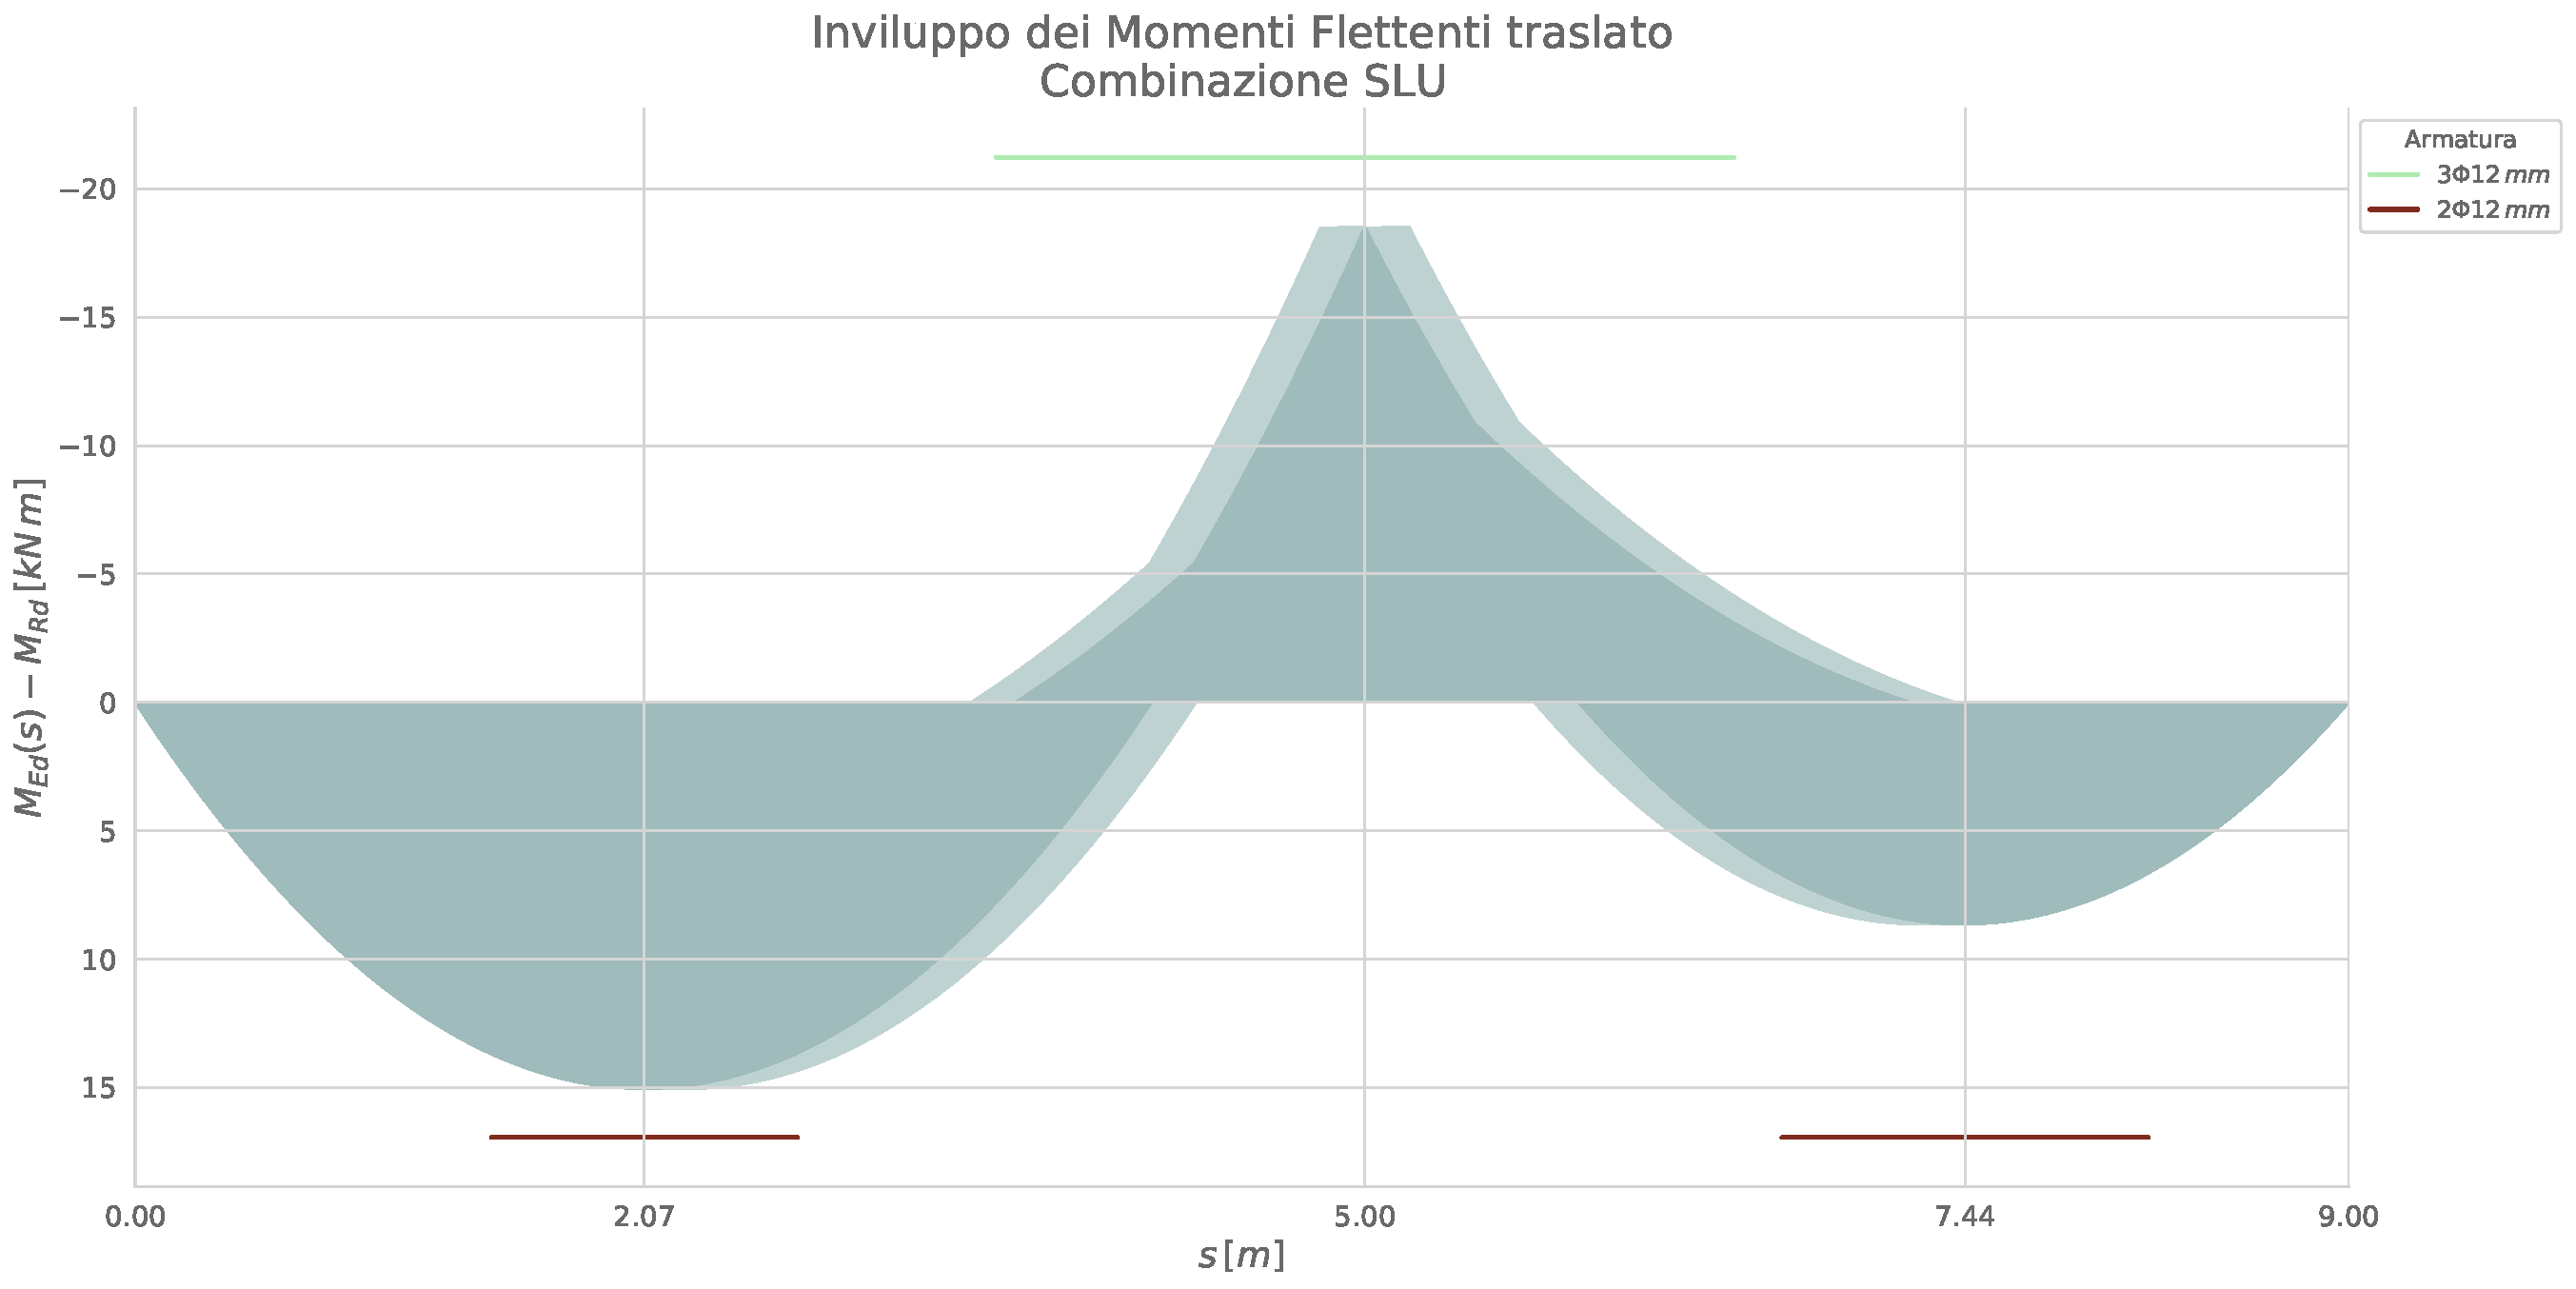
\includegraphics[width=\textwidth]{MEd-MRd_traslato_solaio}
	\caption{Diagramma di inviluppo dei momenti flettenti traslato -- solaio}
	\label{fig:MEd-MRd_traslato_solaio}
\end{figure}

\section{Lunghezza di ancoraggio}\label{sec:ancoraggio_solaio}
In analogia a quanto effettuato per la trave al punto~\ref{sec:ancoraggio}, si calcolano le lunghezze di ancoraggio delle barre per i travetti del solaio. La formula che governa il problema è la medesima a quella della trave e deriva dalla normativa europea. Nell'ipotesi di buona aderenza e assumendo, a favore di sicurezza, che la tensione di lavoro dell'armatura sia pari a $f_{yd}$ si ottengono i seguenti valori:

\begin{align*}
	f_{ctd} &= 1.02\,MPa\\
	\eta_1 &= \eta_2 = 1\\
	f_{bd} &= 2.25\,\eta_1\,\eta_2\,f_{ctd} = 2.30\,MPa\\
	\sigma_{sd} &= f_{yd}\\
	l_{b,rqd} &= \dfrac{\Phi}{4}\,\dfrac{\sigma_{sd}}{f_{bd}} = \dfrac{12}{4}\,\dfrac{391.30}{2.30} \simeq510\,mm \\
	l_{b,min} &\geq \begin{cases}
		\max\{0.3\,l_{b,rqd}; 10\,\Phi; 100\,mm\} \simeq 155\,mm \quad \text{per armature tese}\\
		\max\{0.6\,l_{b,rqd}; 10\,\Phi; 100\,mm\} \simeq 310\,mm \quad \text{per armature compresse}
	\end{cases}\\
	\alpha_1 &= \alpha_3 = \alpha_4 = \alpha_5 = 1 \\
	a &= \dfrac{b - 2\,c-n\,\Phi}{n-1} = \dfrac{120-20-36}{2}\,mm = 32\,mm\\
	c_d &= \min\left\{\dfrac{a}{2}; c_1; c\right\} = 10\,mm\\
	\alpha_2 &= 1-0.15\,\dfrac{c_d - \Phi}{\Phi} = 1.01 \nless 1 ~ \Longrightarrow~ \alpha_2 = 1\\
	l_{bd} &= \alpha_1\,\alpha_2\,\alpha_3\,\alpha_4\,\alpha_5\,l_{b,rqd} = 510\,mm  > l_{b,min} = \begin{cases}
		155\,mm \quad \text{per armature tese}\\                                                                                              
		310\,mm \quad \text{per armature compresse}                                                                                              \end{cases}
\end{align*}

\begin{figure}
	\centering
	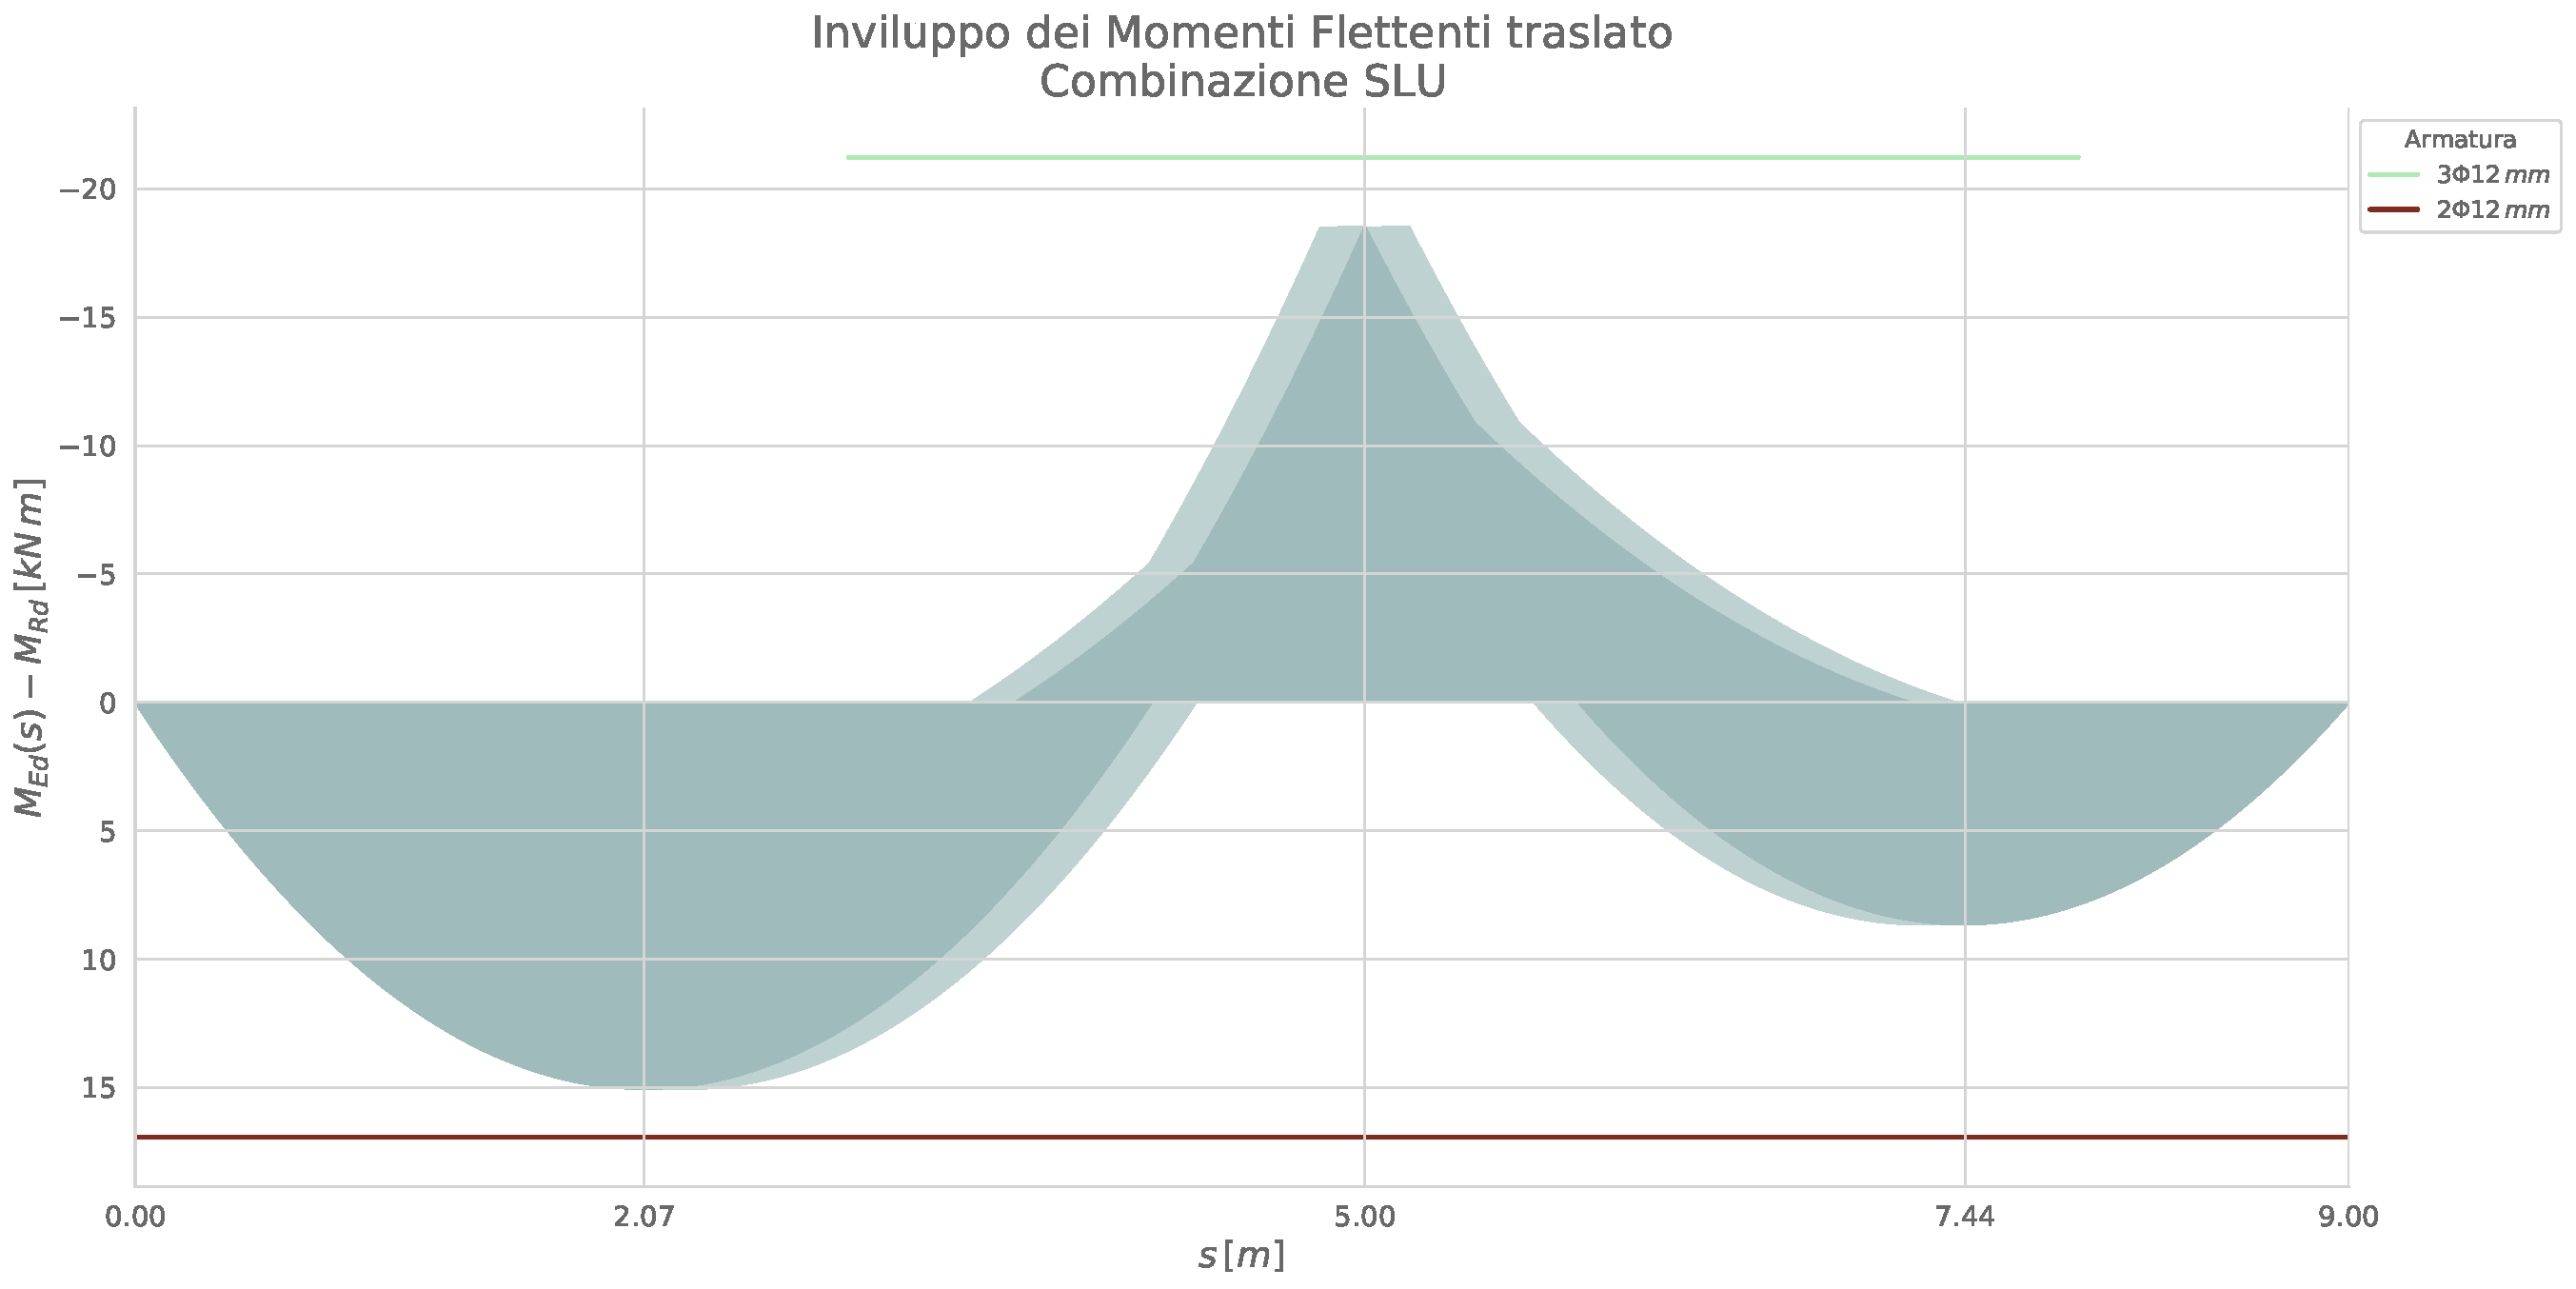
\includegraphics[width=\textwidth]{MEd-MRd_ancoraggi_solaio}
	\caption{Diagramma di inviluppo dei momenti flettenti considerando le lunghezze di ancoraggio -- solaio}
	\label{fig:MEd-MRd_ancoraggi_solaio}
\end{figure}

In figura~\ref{fig:MEd-MRd_ancoraggi_solaio} le armature inferiori sono state prolungate fino all'appoggio centrale, mentre le barre superiori in prossimità dell'appoggio sono state prolungate della lunghezza di ancoraggio sopra calcolata partendo dal punto di nullo del diagramma di inviluppo dei momenti traslato.

\section{Armatura integrativa superiore agli appoggi esterni}
La schematizzazione effettuata sui vincoli alle estremità  -- considerati come dei semplici appoggi -- può essere utile in prima approssimazione per il progetto a flessione del solaio, ma non rispecchia affatto la realtà; la trave presente al bordo difficilmente si può considerare come una cerniera poiché è caratterizzata da una rigidezza torsionale che genera momento flettente che tende le fibre superiori del solaio. Per ovviare al problema è necessario considerare un momento applicato sui vincoli estremi pari a
\[
\dfrac{Q_{Ed,slu}\,l^2}{16\div 20}
\]
dove $Q_{Ed, slu}$ è il valore di carico di progetto riferito alla campata adiacente all'appoggio considerato. In particolare, i carichi agenti su un travetto valgono
\begin{align*}
	Q_{Ed,slu}^{CS1} =Q_{Ed,slu}^{CS2}= 7.05\,\dfrac{kN}{m}
\end{align*}
perciò i momenti agenti sul singolo travetto sono
\begin{align*}
	M_{Ed,slu}^{NS1} &=\dfrac{Q_{Ed,slu}^{CS1}\,l_{CS1}^2}{16} = 11.02\,kN\,m\\
	M_{Ed,slu}^{NS3} &= \dfrac{Q_{Ed,slu}^{CS2}\,l_{CS2}^2}{16} = 7.05\,kN\,m
\end{align*}
tendente le fibre superiori del travetto.

\subsubsection{Progetto NS1}
Supponendo la crisi lato acciaio e la sezione in campo 2 con $\epsilon_c \in [\epsilon_{c2}, \epsilon_{cu}]$ si ottiene il seguente sistema di equazioni
\[
\begin{cases}
	b\,\psi\,\xi\,d\,f_{cd} - A_s\,f_{yd} = 0\\\\
	b\,\psi\,\xi\,d\,f_{cd}\,(d - \lambda\,\xi\,d) = M_{Ed,slu}^{NS1}\\\\
	\psi = \dfrac{16\xi -1}{15\xi}\\\\
	\lambda = \dfrac{171\xi^2 - 22\xi +1}{20\xi\,(16\xi-1)}    
\end{cases}
\]
e sostituendo i valori numerici $b = 120\,mm$, $d=200\,mm$, etc., si ottengono i seguenti risultati
\[
\begin{cases}
    \xi = 0.2299\\
	x = \xi\,d = 45.98\,mm\\
	\epsilon_c = \epsilon_{su}\,\dfrac{\xi}{1-\xi} = 2.985\,\permil \in [\epsilon_{c2}, \epsilon_{cu}]\\
	A_s = 155.184\,mm^2	
\end{cases}
\]
da cui si sceglie un'armatura aggiuntiva superiore pari a
\[
    A_s = 2\,\Phi\,12\,mm = 72\,\pi\,mm^2 = 226.195\,mm^2
\]

\subsubsection{Progetto NS3}
Sull'appoggio estremo a destra si considera la sezione in campo 2 con $\epsilon_c \leq \epsilon_{c2}$. Il sistema lineare si riduce a 
\[
\begin{cases}
	b\,\psi\,\xi\,d\,f_{cd} - A_s\,f_{yd} = 0\\\\
	b\,\psi\,\xi\,d\,f_{cd}\,(d - \lambda\,\xi\,d) = M_{Ed,slu}^{NS3}\\\\
	\psi = \dfrac{5\xi\,(3-8\xi)}{3\,(\xi-1)^2}\\\\
	\lambda = \dfrac{9\xi-4}{4\,(8\xi-3)}    
\end{cases}
\]

Risolvendo in $\xi$ e $A_s$ si ottiene
\[
\begin{cases}
	\xi = 0.1661\\
	x = \xi\,d = 33.23\,mm\\
	\epsilon_c = \epsilon_{su}\,\dfrac{\xi}{1-\xi} = 1.993\,\permil <\epsilon_{c2}\\
	A_s = 96.065\,mm^2	
\end{cases}
\]

Si scelge la seguente armatura
\[
A_s = 1\,\Phi\,12\,mm = 36\,\pi\,mm^2 = 113.10\,mm^2
\]

\section{Armatura integrativa inferiore sugli appoggi}
L'armatura integrativa inferiori deve essere progettata in modo tale da assorbire il taglio di progetto sugli appoggi. 

\subsubsection{Progetto NS1}
Il taglio di progetto sul primo appoggio è di 
\[
V_{Ed}^{NS1} = \dfrac{29.11\,kN}{2} = 14.56\,kN
\]
che deve essere assorbito dall'armatura integrativa. Il numero di barre necessarie, supponendo di usare un diametro $12\,mm$ - arrotondando al numero intero superiore - è
\[
\lceil n \rceil = \left\lceil\dfrac{V_{Ed}^{NS1}}{A_s(12\,mm)\,f_{yd}}\right\rceil = 1
\]
che ha una resistenza a trazione di
\[
n\,A_s\,f_{yd} = 44.26\,kN > V_{Ed}^{NS1}
\]

\subsubsection{Progetto NS2}
Il taglio massimo sull'appoggio centrale vale - in modulo -
\[
V_{Ed}^{NS2} = \dfrac{42.65\,kN}{2} = 21.33\,kN
\]
che implica un'armatura aggiuntiva di
\[
\lceil n \rceil = \left\lceil\dfrac{V_{Ed}^{NS2}}{A_s(12\,mm)\,f_{yd}}\right\rceil = 1
\]
che generano una resistenza a trazione di $44.26\,kN$.

\subsubsection{Progetto NS3}
Il taglio agente sull'appoggio estremo di destra vale
\[
V_{Ed}^{NS3} = \dfrac{22.04\,kN}{2} = 11.02\,kN
\]

Il numero di barre necessarie è di $1\,\Phi\,12\,mm$ come sugli appoggi precedenti.

\section{Verifica a taglio}\label{sec:shearSolaio}
Come anticipato, nel solaio non è possibile inserire armatura resistente a taglio; si deve confidare totalmente sull'effetto pettine sviluppato dalla sezione a $'T'$, che dovrà assorbire il taglio sollecitante di progetto (i cui valori sono riportati nella tabella~\ref{tab:shear_solaio}). Utilizzando un procedimento 'matriciale' - raggruppando quindi i valori riferiti agli appoggi in un vettore - e seguendo quanto descritto nelle \ntc si calcola il taglio resistente di progetto (dalla \textbf{[4.1.22]}) da cui si ottiene
\[
\underline{V_{Rd}} = 
\begin{Bmatrix}
	16.51\\
	18.90\\
	18.90\\
	16.51
\end{Bmatrix}\,kN > \underline{V_{Ed}} = 
\begin{Bmatrix}
	14.55\\
	21.31\\
	18.71\\
	11.01
\end{Bmatrix}
\]



La disuguaglianza è verificata ovunque tranne sull'appoggio $NS2$ lato sinistro, dove il taglio resistente è inferiore al taglio sollecitante
\[
V_{Rd}^{NS2^{sx}} = 18.90\,kN < \left|V_{Ed}^{NS2^{sx}}\right| = 21.31\,kN
\]

In questo caso, non potendo inserire armatura che assorba il taglio necessario si toglie una fila di pignatte (a sinistra dell'appoggio) e si getta un elemento pieno in calcestruzzo. La base da utilizzare durante il calcolo dell'effetto pettine è 
\[
b_w = B                                                                                                                                                                                                                                                                                                                                                                                                                                                                                                                  \]

Il taglio resistente riferito all'appoggio $NS2$ lato sinistro con questa configurazione è
\begin{align*}
	\begin{cases}
		V_{Rd}^{NS2^{sx}} = \max\left\{\left[\dfrac{0.18\,k\,\left(100\,\rho_1\,f_{ck}\right)^{1/3}}{\gamma_c} + 0.15\,\sigma_{cp}\right]\,B\,d; (\nu_{min} + 0.15\,\sigma_{cp})\,B\,d\right\}\\
		k = \min\left\{ 1+\left(\dfrac{200}{d}\right)^\frac{1}{2}; 2\right\}\\
		\rho_1 = \min\left\{\dfrac{A_{sl}}{B\,d}; 0.02\right\}\\
		\sigma_{cp} = \min\left\{\dfrac{N_{Ed}}{A_c}; 0.2\,f_{cd}\right\} = 0\\
		\nu_{min} = 0.035\,k^{\frac{3}{2}}\,f_{ck}^{\frac{1}{2}}
	\end{cases}
\end{align*}

Risolvendo si ottiene
\[
V_{Rd}^{NS2^{sx}} = 48.95\,kN > \left|V_{Ed}^{NS2^{sx}}\right| = 21.33\,kN
\]

La sovrapposizione tra il diagramma del taglio sollecitante di progetto e il taglio resistente nei due casi è rappresentata nelle figure~\ref{fig:VEd-VRd_solaio_slu} e \ref{fig:VEd-VRd_solaio_corretto}.

\begin{figure}
	\centering
	\subfloat[\emph{Confronto tra taglio sollecitante e taglio resistente}]{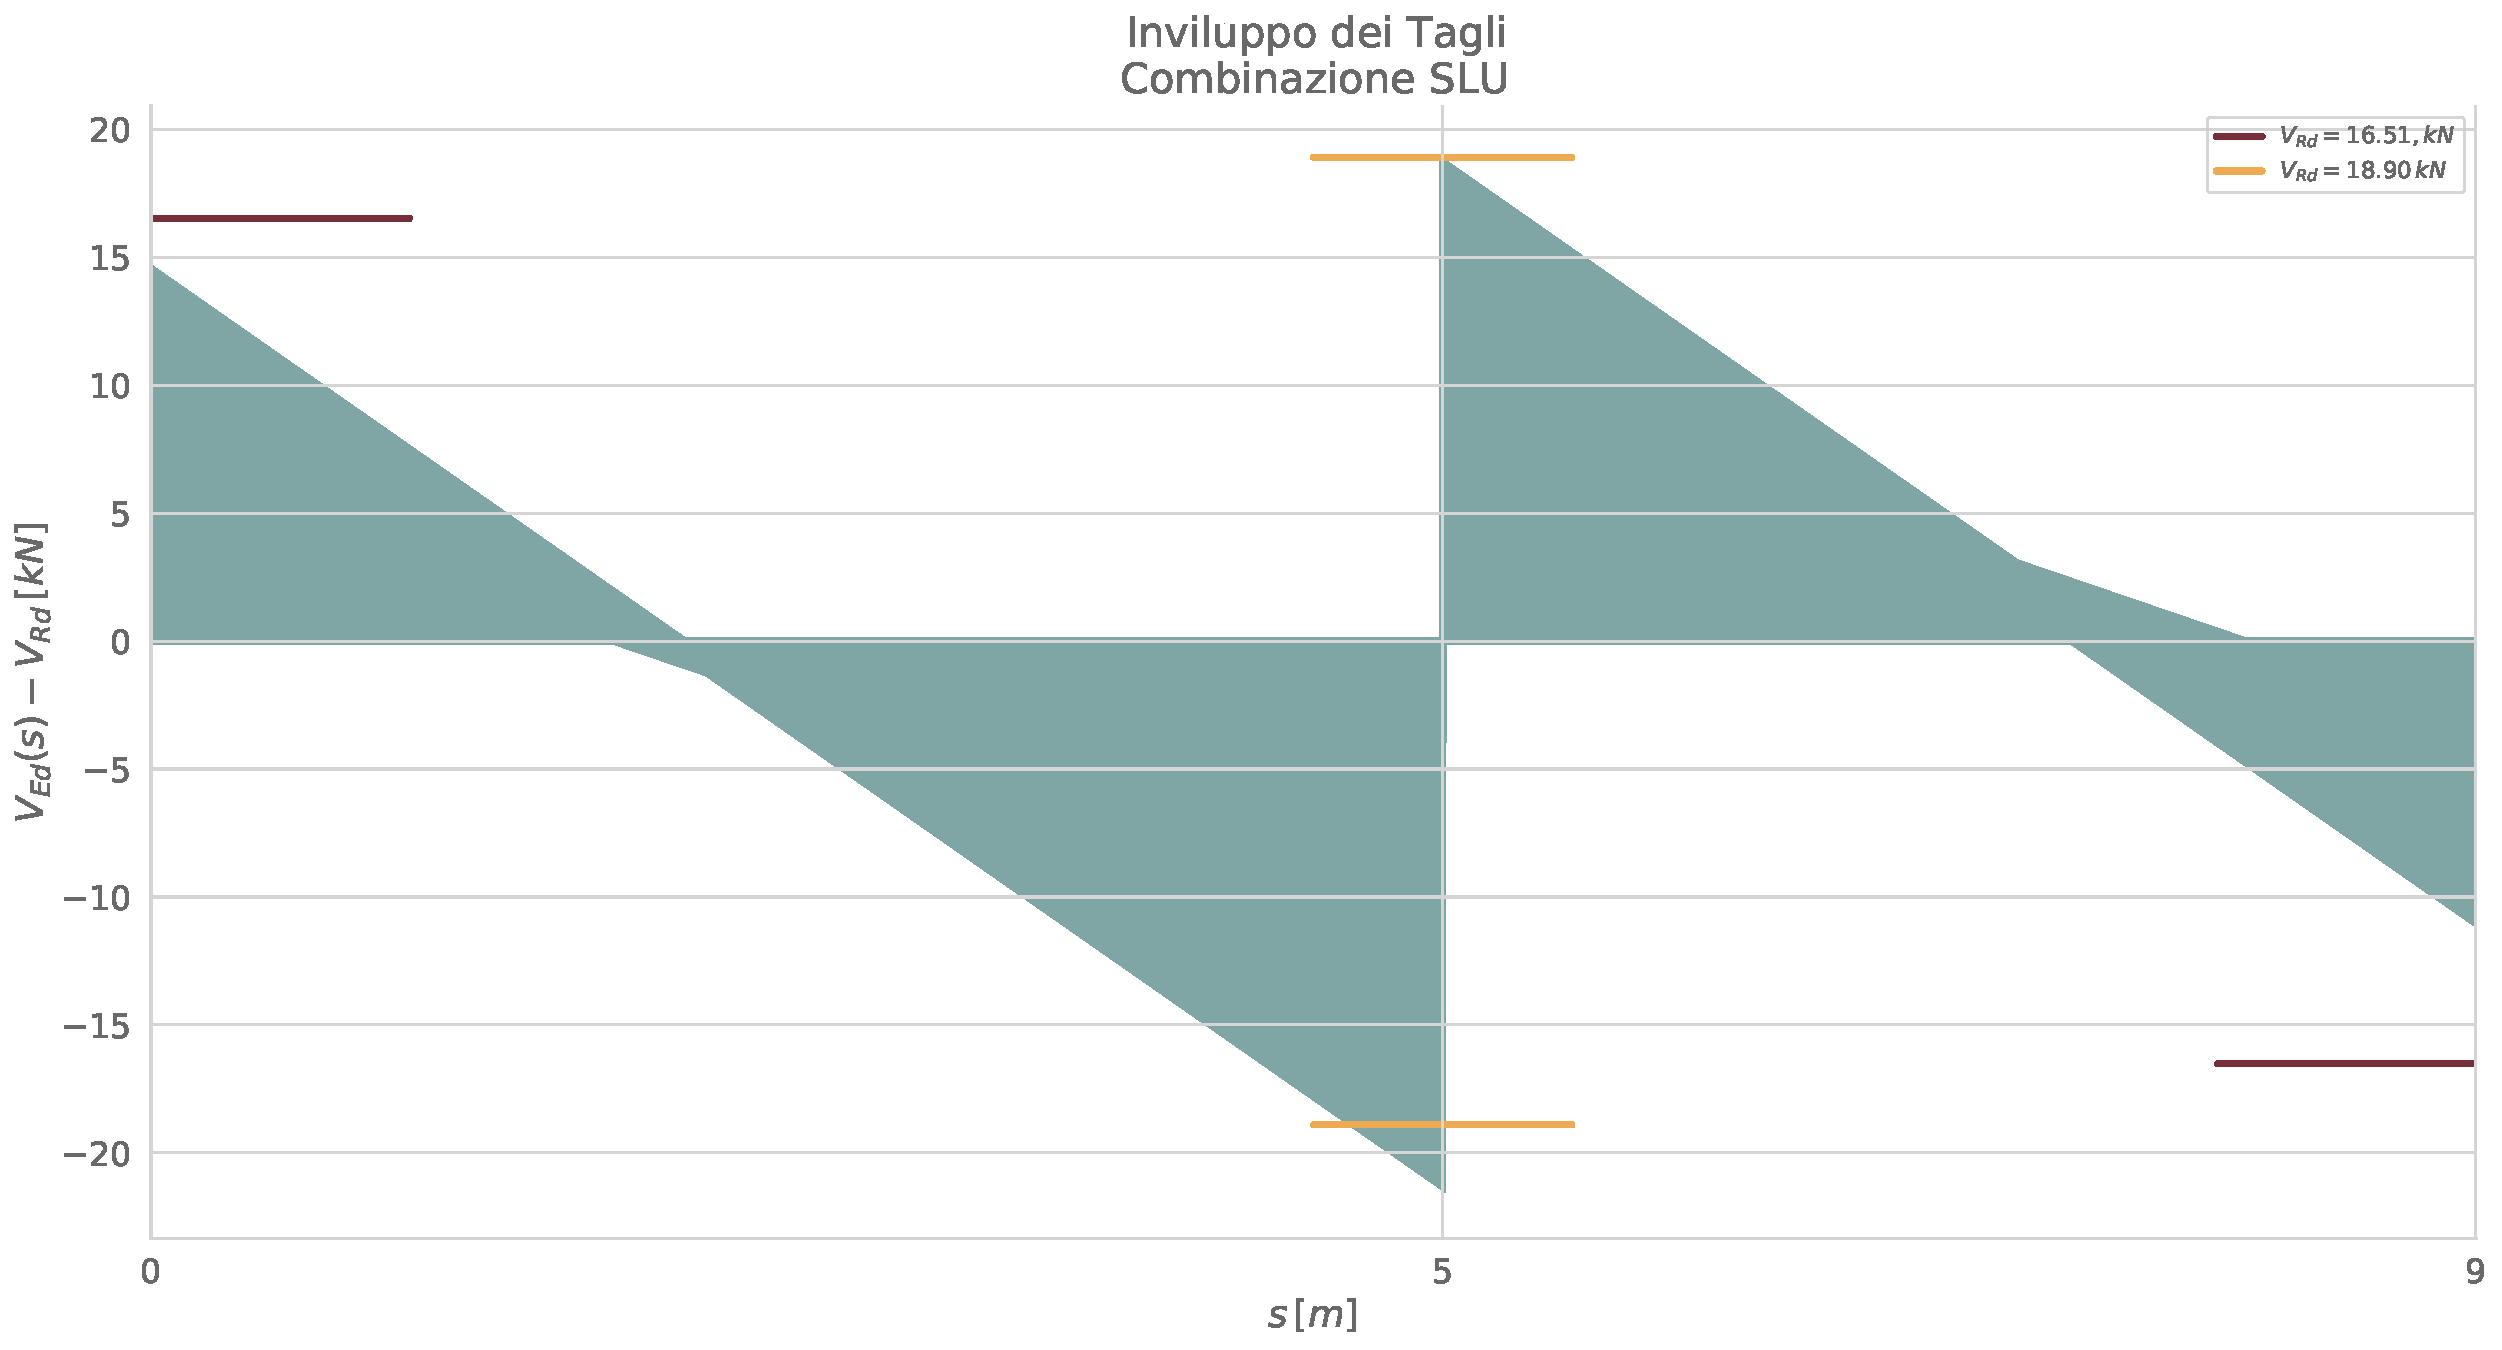
\includegraphics[width=\textwidth]{VEd-VRd_solaio_slu}\label{fig:VEd-VRd_solaio_slu}}\\
	\subfloat[\emph{Confronto tra taglio sollecitante e taglio resistente togliendo una fila di pignatte}]{
		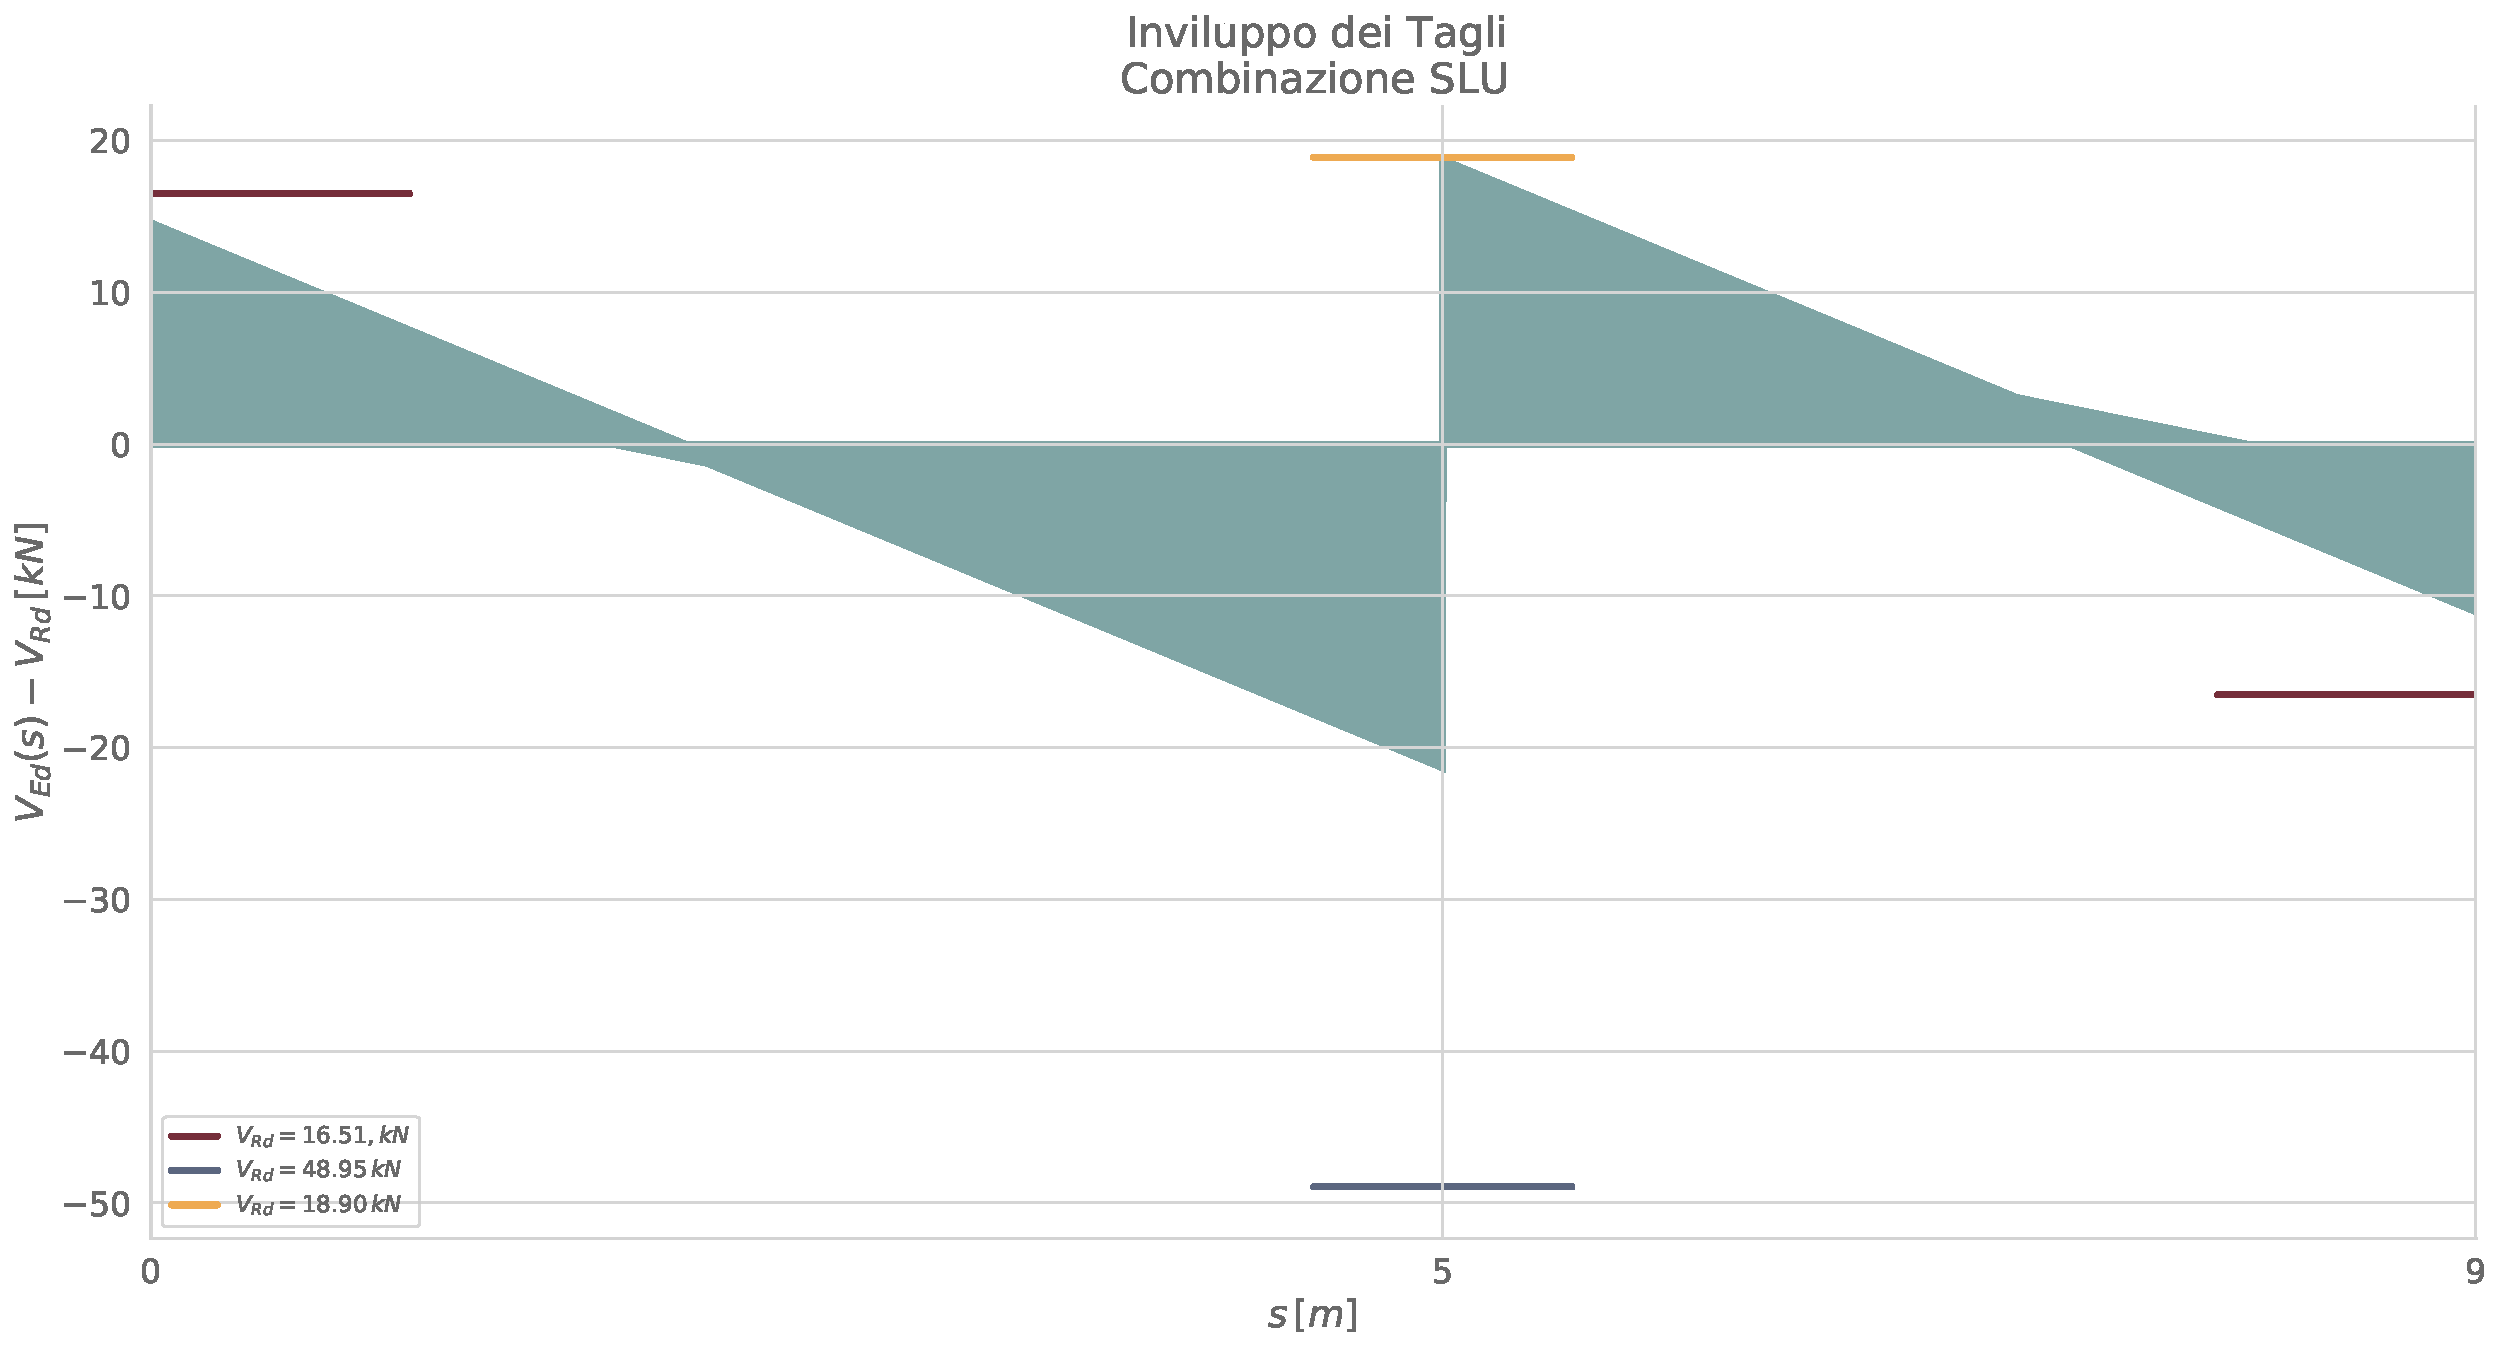
\includegraphics[width=\textwidth]{VEd-VRd_solaio_corretto}\label{fig:VEd-VRd_solaio_corretto}}
	\caption{$V_{Ed} - V_{Rd}$}
	\label{fig:VEd-VRd_solaio}
\end{figure}


